% !TeX spellcheck = es_PE-SpanishPeru
\subsection*{Fuerzas}
\subsubsection*{Fuerza de acción - fuerza ejercida o realizada}
Son aquellas fuerzas de acción que se encuentran o actúan sobre una partícula. Estas fuerza suelen darse en problemas de física I como datos o incógnitas.
\subsubsection*{Fuerza de gravedad - peso}
La fuerza de gravedad, es aquella fuerza de atraccion que ejerce un cuerpo sobre otro y se denota por $F_g$.
\begin{Theorem*} {Ley de gravitación universal}
	Sean dos particulas o sistema de particula, su fuerza de atraccion entre ambos, se define de la siguiente manera:
	$$ \vb{F}_G=G\frac{m_1m_2}{r^2} $$
	donde G es la constante de gravitación universal.
\end{Theorem*}
Sin embargo en nuestro caso tomaremos g como una constante lo que conyeva que la ecuacion de la fuerza de gravedad se simplifique.
\begin{Theorem*} {Fuerza de gravedad - gravedad constante}
	Sí la gravedad permanece constante durante todo el estudio entonces, la fuerza de la gravedad se define de la siguiente manera:
	$$ \vb{a}_G=m\cdot g $$
\end{Theorem*}
donde el valor de la gravedad comunmente es: $g=9.81[m/s^2]$ o $g=32.2[ft/s^2]$.
\subsubsection*{Fuerzas de reaccion}
Son aquellas fuerzas que surgen como una fuerza reciproca a otra fuerza. Es decir que ser originan como respuesta o reacción a otra fuerza que realiza la acción. \\
Algunas fuerza de reacción son la fuerza normal y fuerza de rozamiento, sin embargo en ocasiones suele representarse a todas las fuerzas de reacción como una sola fuerza llamada solamente reacción y representada por una $R$.
\subsubsection*{Fuerza normal}
Es una fuerza de contacto entre dos cuerpos que obra en dirección perpendicular a la superficie común de contacto.
\begin{figure}[H]
	\centering
	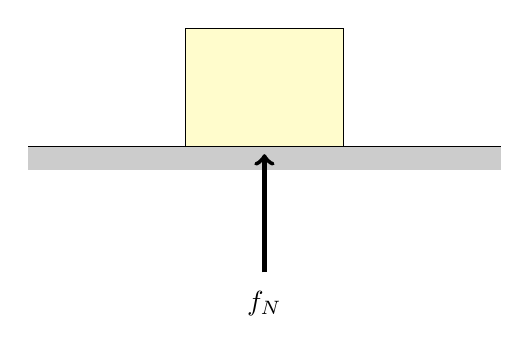
\begin{tikzpicture}
		\draw[draw=black,fill=yellow!20] (-1,1.5) rectangle (1,0);
		\draw[draw=none,fill=black!20] (-3,0) rectangle (3,-0.3);
		\draw (-3,0) -- (3,0);
		\draw[ultra thick,->] (0,-1.6) -- (0,-0.1);
		\node at (0,-2) {$f_N$};
	\end{tikzpicture}
\end{figure}
\begin{figure}[H]
	\centering
	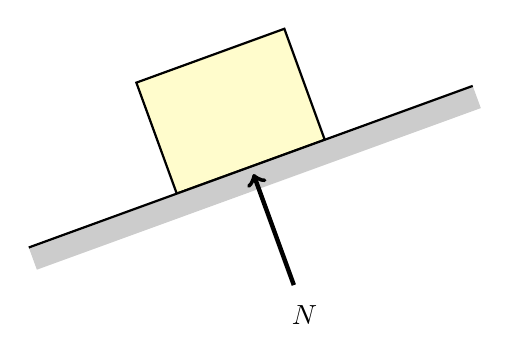
\begin{tikzpicture}[rotate=20,thick]
		\draw[draw=black,fill=yellow!20] (-1,1.5) rectangle (1,0);
		\draw[draw=none,fill=black!20] (-3,0) rectangle (3,-0.3);
		\draw (-3,0) -- (3,0);
		\draw[ultra thick,->] (0,-1.6) -- (0,-0.1);
		\node at (0,-2) {$N$};
	\end{tikzpicture}
\end{figure}
\begin{figure}[H]
	\centering
	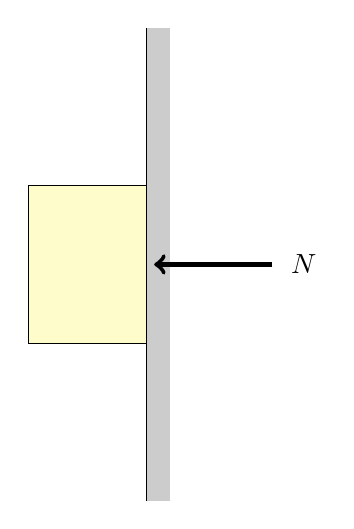
\begin{tikzpicture}[rotate=90]
		\draw[draw=black,fill=yellow!20] (-1,1.5) rectangle (1,0);
		\draw[draw=none,fill=black!20] (-3,0) rectangle (3,-0.3);
		\draw (-3,0) -- (3,0);
		\draw[ultra thick,->] (0,-1.6) -- (0,-0.1);
		\node at (0,-2) {$N$};
	\end{tikzpicture}
\end{figure}
\subsubsection*{Fuerza de tension}
Es una fuerza a distancia entre dos particulas, esta fuerza aplica a atraves de una ligadura (cuerda), suele simbolizarse por una $T$.
\begin{figure}[H]
	\centering
	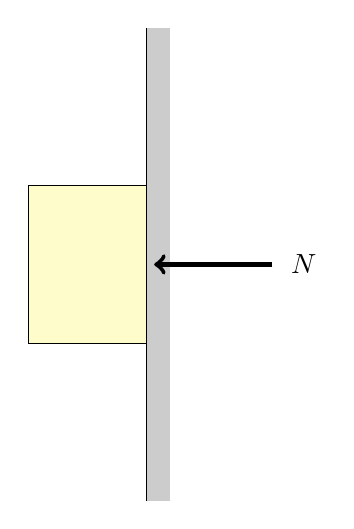
\begin{tikzpicture}[rotate=90]
		\draw[draw=black,fill=yellow!20] (-1,1.5) rectangle (1,0);
		\draw[draw=none,fill=black!20] (-3,0) rectangle (3,-0.3);
		\draw (-3,0) -- (3,0);
		\draw[ultra thick,->] (0,-1.6) -- (0,-0.1);
		\node at (0,-2) {$N$};
	\end{tikzpicture}
\end{figure}
\subsubsection*{Fuerza de tensión}
Es una fuerza a distancia entre dos partículas, esta se aplica a través de una ligadura (cuerda), que normalmente en problemas de partículas despreciamos su masa. Suele simbolizarse por una T.
\begin{figure}[H]
	\centering
	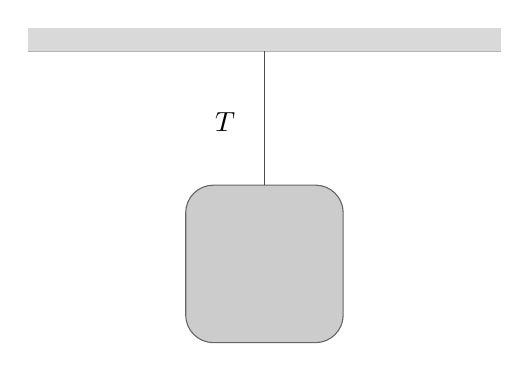
\begin{tikzpicture}
		\draw [draw=none,fill=black!15] (-3,0) rectangle (3,-0.3);
		\draw [black!30,] (-3,-0.3) -- (3,-0.3);
		\draw [black!60,fill=black!20,rounded corners=10pt] (-1,-2) rectangle (1,-4);
		\draw [black!70] (0,-0.3) -- (0,-2);
		\node at (-0.5,-1.2) {$T$};
	\end{tikzpicture}
\end{figure}
La tensión puede cambiar dependiendo de la polea:

\subsubsection*{Fuerza de rozamiento}
Es una fuerza de reaccion que suele representarse con un $f$, sin embargo